Sensor data fusion is an emerging research field with the aim to combine information from multiple and diverse sources (e.g. different sensors such as thermal and visible cameras, laser, \gps, accelerometer etc.) to achieve inferences that cannot be obtained from a single sensor or source, or whose quality exceeds that of an inference drawn from any single source \cite{bonnifait2001data, koneru2011fuzzy}. Sensor data fusion is a multi-disciplinary subject that overlaps with areas like statistical estimation, signal processing, computer vision machine learning etc. In computer vision familiarly image sensor is fused with other sensors in order to develop an intelligent 
system. Now days cameras are cheap small and ubiquitous, and with the emergence of energy-efficient and powerful processors, it has become possible to incorporate practical computer vision and machine learning capabilities into embedded systems, mobile devices etc. \par
Localization is a fundamental problem associated with autonomous navigation. One of the simplest solution to the localization problem is with the help of Global Positioning Systems(\gps). In literature, computer vision methods have also been successfully used for predicting the location. A wide variety of modern gadgets (e.g. smartphones) have both \gps and vision sensors, and such devices are becoming increasingly affordable for low cost robotic systems. Each sensor has its own unique characteristics and its challenges. Unfortunately, the accuracy of the popular \gps tracking devices are limited to only 10$\sim$20 meters, which is insufficient for many robotic tasks\cite{hays2008im2gps}. So noise in the \gps signal becomes a significant issue if we want a reliable localization performance. Where as vision based localization methods suffers problems like occlusion, perceptual aliasing etc. Hence we can deduce for reliable localization fusing multiple sensors which are complimentary in nature will lead us to more accurate and robust localization. The ambiguities in visual localization can be reduced with the help of \gps. Similarly, noise in the \gps signal can be reduced by looking at the visual consistency across multiple sessions. We empirically validate our solution and show that fusing of \gps and camera sensors which are having complementary advantages and disadvantage can result in a more accurate and reliable localization. \par
Smartphones have become essential part of our daily life as they continue to evolve and introduce newer features. However battery capacity of smart phones have failed to keep up the pace at which smartphones have evolved in recent years. It was observed that the network services like Wi-Fi, EDGE and 3G are most power consuming process on the smartphones \cite{carroll2010analysis}. Hence, reducing the power consumption by these processes could help in power savings. Using the significant data from different sensors like accelerometer, touch and system usage we propose a novel approach to schedule services like Wi-Fi and 3G on smartphones. Different sensors data were fused to model and monitor the user activity level to decide when the wireless data module should be turned off for maximal energy saving. Taking Wi-Fi as an example, we show that intelligent scheduling of the Wi-Fi service based on a users activity level leads to lower power consumption without adversely affecting the user experience. \par
\begin{figure}[h]
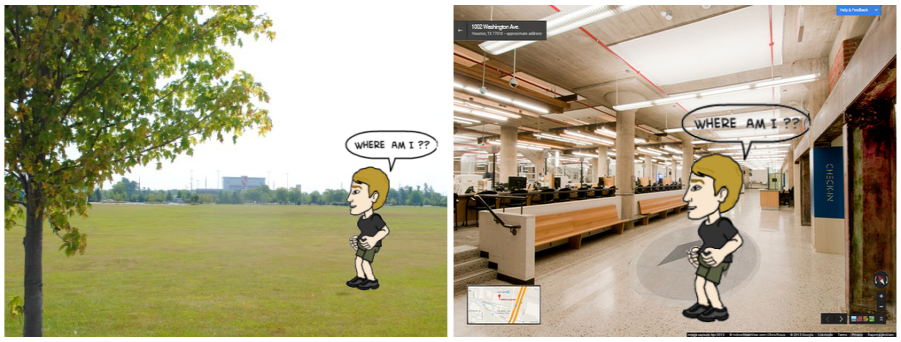
\includegraphics[width=\columnwidth,height=6cm]{figures/localization.png}
\caption{Localization is a process that determine the position of a
robot/human pedestrians in a given environment.}
\label{fig:localization}
\end{figure}
Computer vision task is notably demanding, for a variety of reasons. First, simply put, there are massive amounts of data to consider. Frame resolutions higher than 1 Mpixel need to be streamed uncompressed at 30 to 60 frames per second, and every pixel of each frame requires processing attention. Typical vision processing algorithms for classification or tracking, for example, also combine a mix of vector and scalar processing steps, which demand intensive external memory access patterns with conventional processing architectures. Shuttling intermediate processing results back and forth between the CPU and external memory drives up power consumption and increases overall processing latency. In recent years have we seen vision capabilities show up in mobile applications. Running these algorithms on mobile device comes up with new set of challenges like optimizing the existing algorithms, good understanding of system in order to handle memory and computational requirement.

We describe the background for the computer vision and machine learning tasks tackled in this thesis in Section \ref{sec:cv_ml_task}.
%In Section 1.2 challenges which need to be addressed while designing %strategies for the computer vision and machine learning tasks are explain.
Problem statement and the technical contributions of this thesis have been presented in Section \ref{sec_prob_statmnt_contrib}.

%----------------------------------------------------------------------
\section{Computer Vision and Machine Learning Concepts} 
\label{sec:cv_ml_task}
\subsection{Content based image retrieval}
Content-based image retrieval (CBIR), also known as query by image content (QBIC) is an application of computer vision techniques to the image retrieval problem, that is, the problem of searching for digital images in large databases \cite{smeulders2000content}. A generic and simple model of a CBIR is shown in Figure \ref{fig:cbir}.
"Content-based" means that the search analyzes the contents of the image rather than the metadata such as keywords, tags, or descriptions associated with the image. Given a query image, its features are extracted and compared with the stored database features and a ranked list of images relevant to the query is retrieved.\\
\begin{figure}
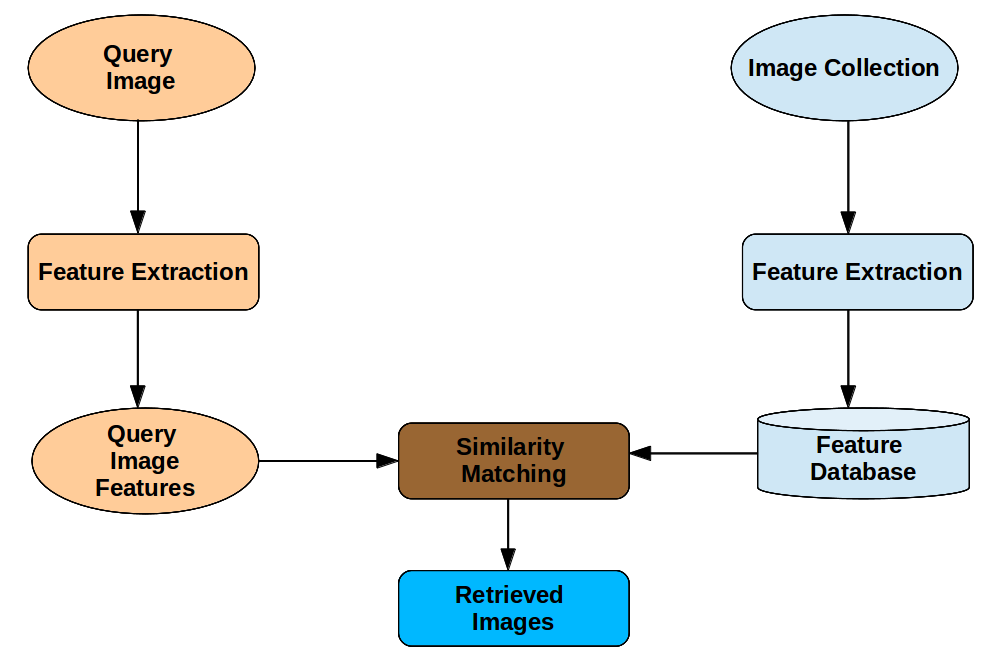
\includegraphics[width=\columnwidth,height=9cm]{figures/img_retrieval.png}
\caption{Figure shows a generic model of Content-based image retrieval system. User can fire the query in form of images in result system return the similar images from the database.}
\label{fig:cbir}
\end{figure}
The CBIR technology has numerous applications like vision based localization, fingerprint identification, biodiversity information systems, digital libraries, crime prevention, medicine,
historical research etc \cite{gudivada1995content}. In this thesis visual localization is formulates as CBIR based problem.
A query image is provided by an image sensor given this single image, we retrieve visually similar images from the database. A voting mechanism is applied on all the retrieved images in order to choose best match
and estimates the location.

\subsection{Classification}
In machine learning, classification is the problem of labeling to which category a new observation belongs to, using the training set of data containing observations whose labels are known to us. A popular example can be for a new incoming e-mail  we have to label it as "spam" or "non-spam". In machine learning,  classification is taken as instance of supervised learning, i.e. learning where a training set of correctly identified observations is available. An algorithm that implements classification at concrete implementation level is known as a classifier. The term "classifier" sometimes also refers to the mathematical function, implemented by a classification algorithm, that labels the input data.
Support Vector Machine(SVM), Decision Tree, Logistic Regression and Naive Base are few famous classification algorithm which are used frequently to perform the classification task.

%In this thesis we have used SVM for to perform the classification task. SVM is supervised learning model it classifies data by finding the best hyperplane that separates all data points of one class from those of the other class. The best hyperplane for an SVM means the one with the largest margin between the two classes(refer Figure \ref{fig:svm_hyperplane}). Margin means the maximal width of the slab parallel to the hyperplane that has no interior data points.In addition to performing linear classification, SVMs can efficiently perform a non-linear classification using a nice mathematical trick called kernel trick, implicitly mapping their inputs into high-dimensional feature spaces.

\subsection{Dimensionality Reduction}
In machine learning dimensionality reduction is the way to reduce the number of random variables under consideration and can be divided into feature selection and feature extraction. Dimensionality reduction is usually performed on higher dimensionality data set in order to avoid curse of dimensionality. Principal component analysis (PCA), linear discriminant analysis (LDA), or canonical correlation analysis (CCA) are
the techniques which can be used to perform the dimensionality reduction.
Figure \ref{fig:pca_dimen} shows a demo example of dimensionality reduction.
\begin{figure}
\centering
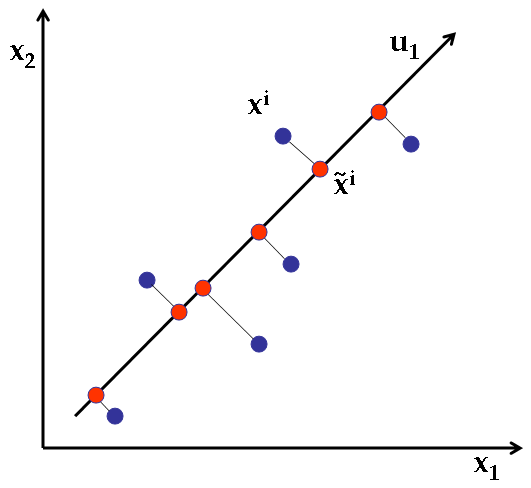
\includegraphics[width=8cm,height=8cm]{figures/pca_example.png}
\caption{Two dimensional data points(blue) are projected along the vector $u_1$(red) in order to reduce the dimensionality.}
\label{fig:pca_dimen}
\end{figure}
 
%\section{Challenges in Computer Vision and Running on Embedded devices}
%\label{sec:challenges_cv_ml_task}
%Most of the computer vision task face a number of challenges occlusion, change in view point, lighting condition of objects, noise in labeled data, image quality etc. To run computer vision algorithms high computational power and memory is required. In recent years have we seen vision capabilities show up in embedded applications. Running these algorithms on embedded device comes up with new set of challenges like
%optimizing the existing algorithms, good understanding of system in order to handle memory and computational requirement.

\section{Problem Statement and Contribution}
\label{sec_prob_statmnt_contrib}
The focus of this thesis is on multi-sensor data fusion. We have shown empirically by fusing data from multiple sources increases the robustness and efficiency of a system. We aim at using the sensors like GPS, camera, accerelometer and touch sensors and demonstrated how they compliment each other. Taking these into consideration, we would like to specifically address the following sub-problems:
\begin{enumerate}
\item \textbf{Improving Localization by Fusing Camera and GPS Sensors:} We addresses the problem of localization by fusing \gps and camera sensor using vision algorithms. Peculiarly we demonstrate how a noisy \gps signal can be amend by vision based localization of images in an environment, alternatively we also show that \gps information can be used as a tie breaker for visually similar looking images but belong to different places. We focus on the challenges like occlusion, change in view point and noise in \gps data and showed by using multiple sensor data we can handle these problems more efficiently as compare to single sensor.  

%\item \textbf{Problem:} \textit{Story telling for a heritage sites. Aim is to build a system which can act as virtual tourist guide for a given heritage site and narrate a story as you move along.\\}
%This work is focused on developing a story telling application on mobile phones using \gps and vision cues. This application builds an immersive experience for participants and wraps a narrative around them according to the surrounding while they leisurely walk around a heritage site.

\item \textbf{Reducing Power Consumption by Fusing Sensors data on Smartphones:} Smartphone are powered from batteries which is limited in their capacity. Services like Wi-Fi and 3G are one of the most power consuming processes on smartphone but one good thing with these services are they are not required in a continuous fashion. To reduce the power consumption by these services we predict the user activity level and make them available only when they are needed. We model the user activity level with respect to smartphone device by fusing different sensors data like accelerometer, touch screen, cpu and memory usage. Based on these levels we schedule the services like Wi-Fi and 3G to reduce the power consumption of the smartphones.
\end{enumerate}

%----------------------------------------------------------------------
\section{Thesis Outline} 
\label{sec_thesis_outline}

In $Chapter \ref{ch:chap2}$, we briefly discuss the technical background needed for the later chapters in the thesis. In $Chapter \ref{ch:chap3}$ the problem of localization by fusing the \gps and image sensors has been tackled. In this chapter we demonstrate how \gps and image sensor can be fused together to overcome the issues like occlusion, perceptual aliasing etc.. $Chapter \ref{ch:chap5}$ shows how sensor data fusion with machine learning algorithm can make the smart devices more smarter and efficient. Using the data from accelerometer, touch sensors, CPU and RAM usage we have tried to predict the user engagement with phone and schedule the Wi-Fi accordingly in order to save the battery power. Conclusions, and future directions of our work have been given in $Chapter \ref{ch:conc}$.

\newpage








